% -*- TeX:de -*-
\NeedsTeXFormat{LaTeX2e}
\documentclass[12pt,a4paper]{article}
\usepackage[german]{babel} % german text
\usepackage[DIV12]{typearea} % size of printable area
\usepackage[T1]{fontenc} % font encoding
%\usepackage[latin1]{inputenc} % most likely on Windows
\usepackage[utf8]{inputenc} % probably on Linux
\usepackage{multicol}

% PLOTTING
\usepackage{pgfplots} 
\usepackage{pgfplotstable}
\usepackage{url}
\usepackage{graphicx} % to include images
\usepackage{tikz}
\usepackage{subfigure} % for creating subfigures
\usepackage{amsmath} % a bunch of symbols
\usepackage{amssymb} % even more symbols
\usepackage{booktabs} % pretty tables
\usepackage{makecell} % multi row table heading

% a floating environment for circuits
\usepackage{float}
\usepackage{caption}

%\newfloat{circuit}{tbph}{circuits}
%\floatname{circuit}{Schaltplan}

% a floating environment for diagrams
%\newfloat{diagram}{tbph}{diagrams}
%\floatname{diagram}{Diagramm}

\selectlanguage{german} % use german

\begin{document}








%%%% TO DO
%
% - - Shorty:
%
% - - Tabelle "Messwerte Linsenbrennweite"
%		bitte bei jedem neuen e eine trennlinie... bin zu deppert ^^

% - - Patrick
%




%%%%%%% DECKBLATT %%%%%%%
\thispagestyle{empty}
			\begin{center}
			\Large{Fakultät für Physik}\\
			\end{center}
\begin{verbatim}


\end{verbatim}
							%Eintrag des Wintersemesters
			\begin{center}
			\textbf{\LARGE WS 2013/14}
			\end{center}
\begin{verbatim}


\end{verbatim}
			\begin{center}
			\textbf{\LARGE{Physikalisches Praktikum\\ für das Bachelorstudium}}
			\end{center}
\begin{verbatim}




\end{verbatim}

			\begin{center}
			\textbf{\LARGE{PROTOKOLL}}
			\end{center}
			
\begin{verbatim}





\end{verbatim}

			\begin{flushleft}
			\textbf{\Large{Experiment (Nr., Titel):}}\\
							%Experiment Nr. und Titel statt den Punkten eintragen
			\LARGE{PW8 Wellenoptik}	
			\end{flushleft}

\begin{verbatim}

\end{verbatim}	
							%Eintragen des Abgabedatums, oder des Erstelldatums des Protokolls
			\begin{flushleft}
			\textbf{\Large{Datum:}} \Large{21.11.2013}
			\end{flushleft}
			
\begin{verbatim}
\end{verbatim}
							%Namen der Protokollschreiber
		\begin{flushleft}
			\textbf{\Large{Namen:}} \Large{Patrick Braun, Johannes Kurz}
			\end{flushleft}

\begin{verbatim}


\end{verbatim}
							%Kurstag und Gruppennummer, zb. Fr/5
			\begin{flushleft}
			\textbf{\Large{Kurstag/Gruppe:}} \Large{DO/2}
			\end{flushleft}

\begin{verbatim}



\end{verbatim}
							%Name des Betreuers, das Praktikum betreute.
			\begin{flushleft}
			\LARGE{\textbf{Betreuer:}}	\Large{ Johanna Akbarzadeh }	
			\end{flushleft}

%%%%%%% DECKBLATT ENDE %%%%%%%
\pagebreak
\setlength{\columnsep}{20pt}
\begin{multicols}{2}


%\begin{figure}[H]
%	\centering
%	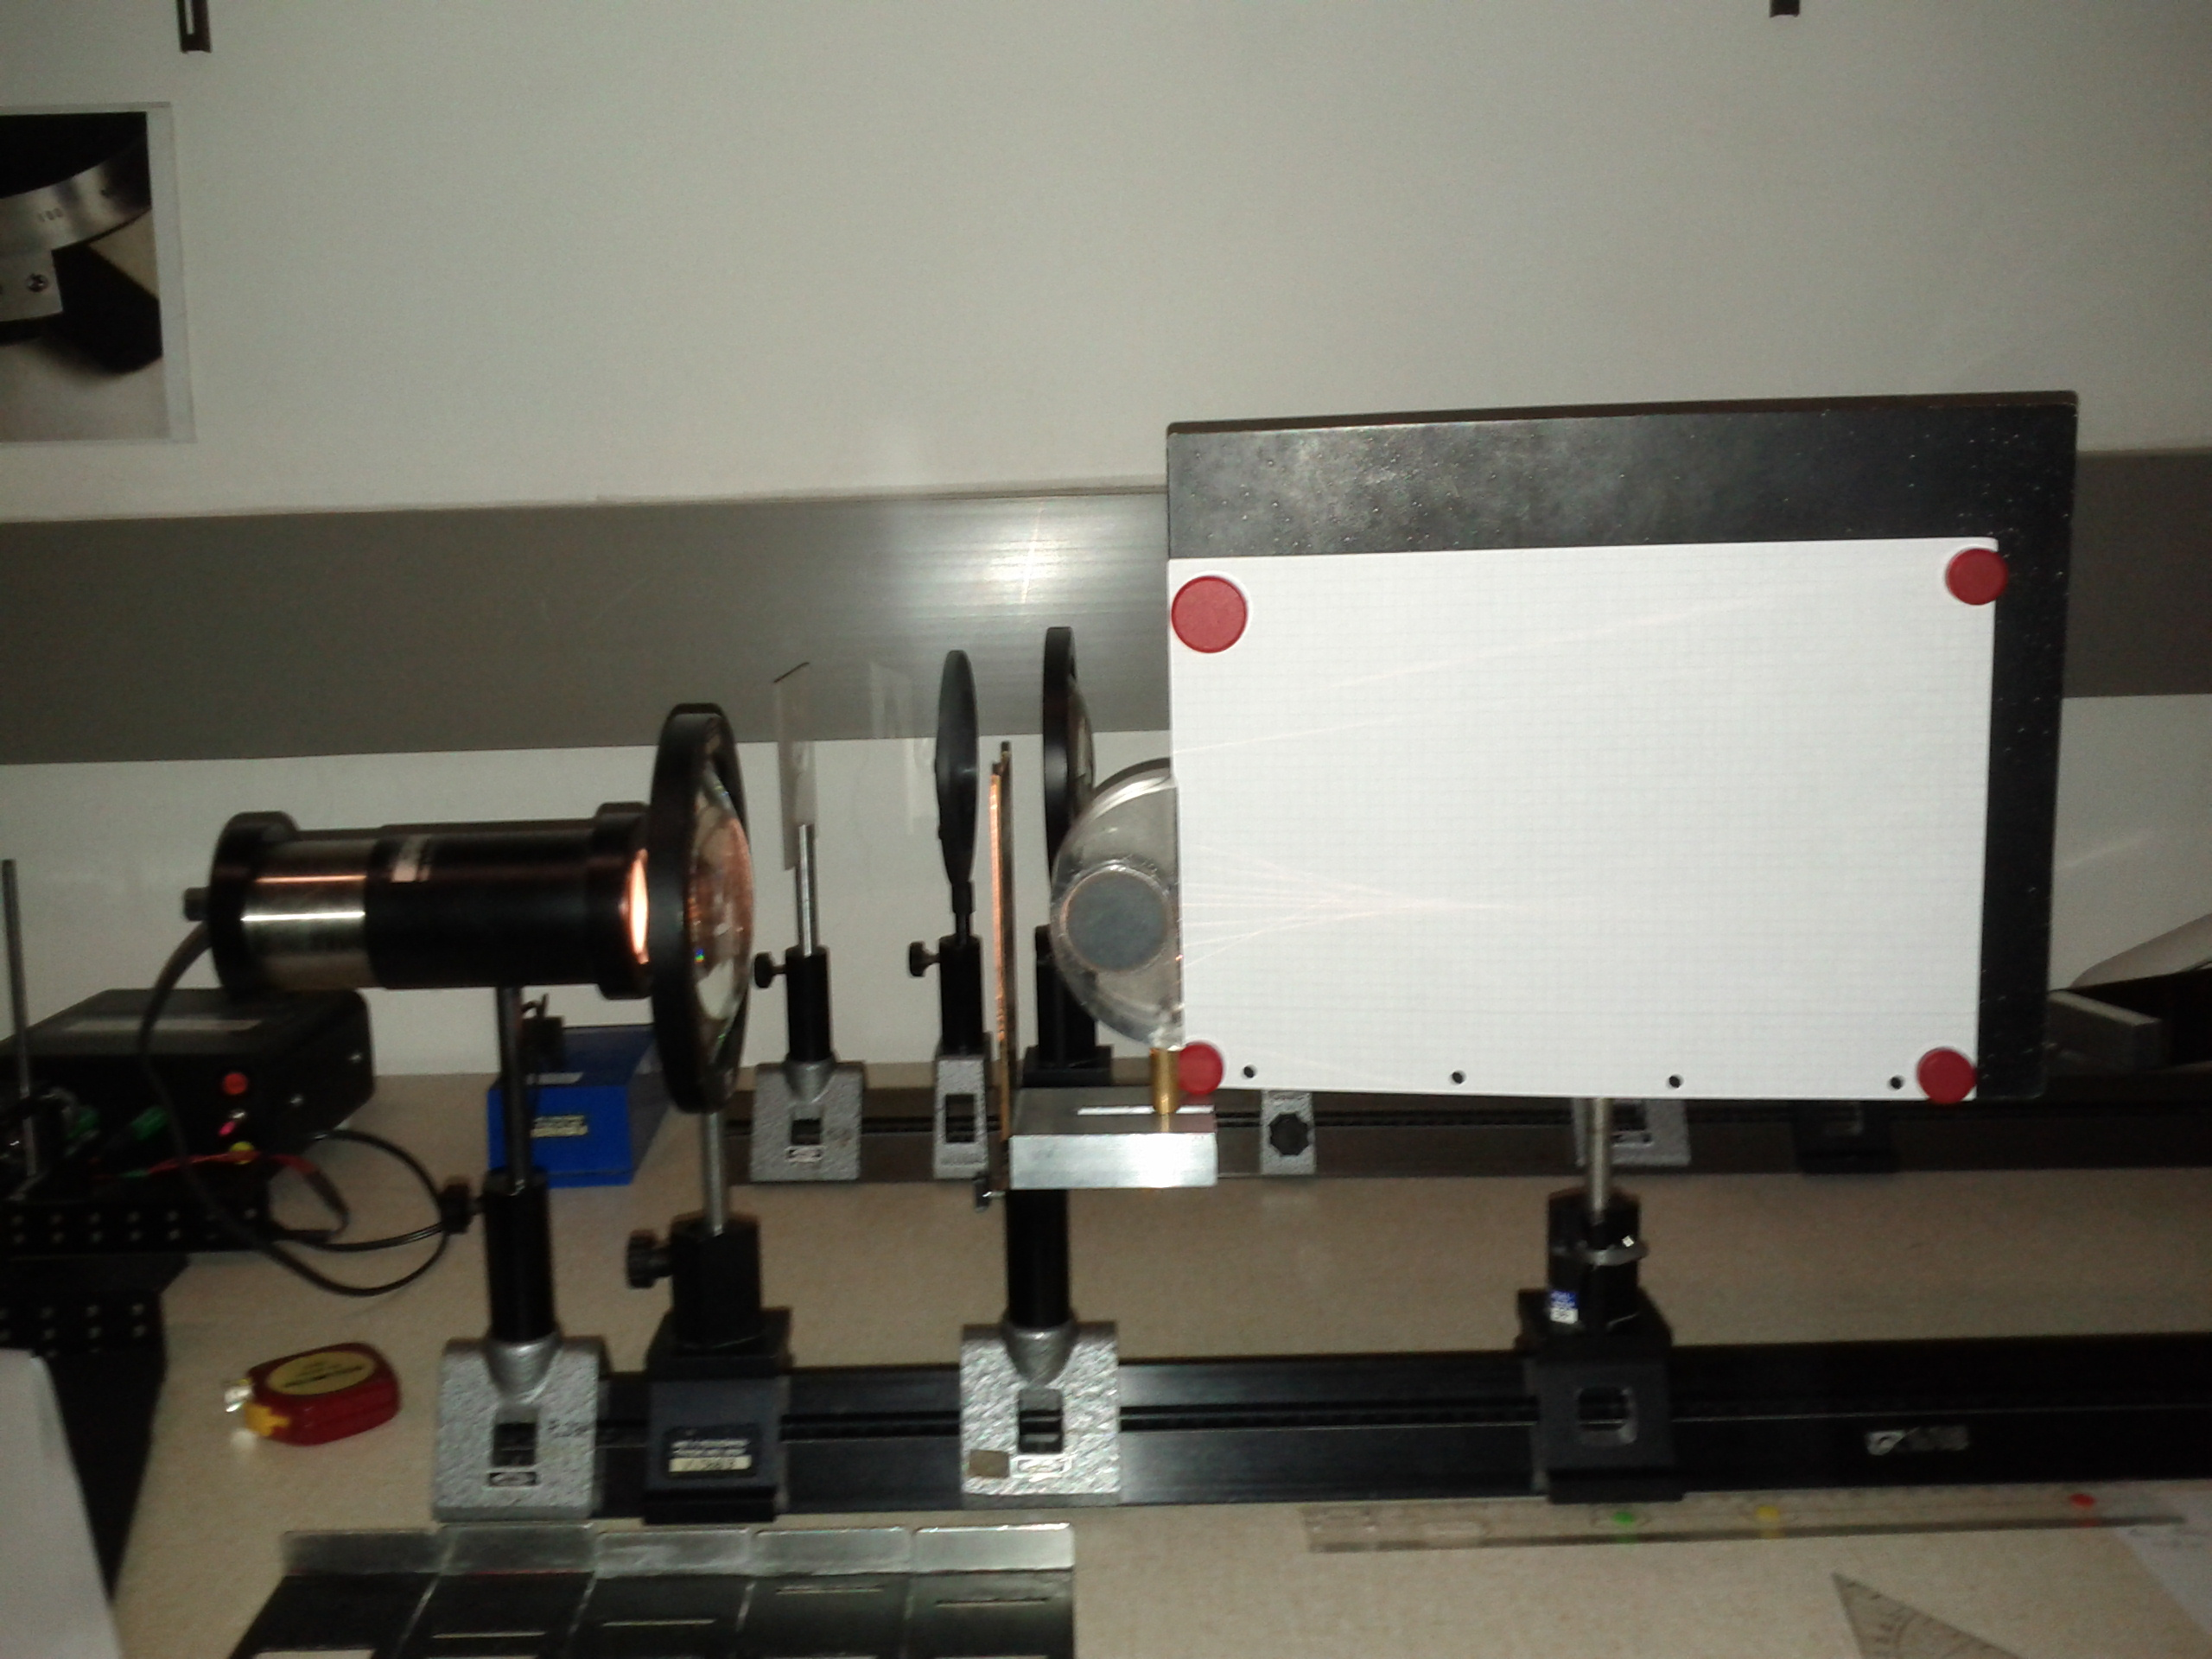
\includegraphics[scale=0.13]{./figure/linsenfehler.jpg}
%	\caption{Versuchaufbau Konvex-Plan Linse}
%	\label{fig:linsenfehler_aufbau}
%\end{figure}
%
%Glasprisma gegen Luft
%1.000292/sin(39grad28minutes)


%\begin{figure}[H]
%	\centering
%	\pgfplotstabletypeset[
%			columns={farbe, w,lambda},
%			col sep=&,
%			columns/farbe/.style={string type, column name=\makecell{$Farbe$\\} }, 
%			columns/w/.style={string type, column name=\makecell{$Winkel$\\$[Grad]$} }, 
%			columns/lambda/.style={column name=\makecell{$Wellenlänge$\\$[nm]$}, precision=0},
%			every head row/.style={before row=\hline,after row=\hline\hline},
%			every last row/.style={after row=\hline},
%			every first column/.style={column type/.add={|}{} },
%			every last column/.style={column type/.add={}{|} }
%			]{
%			farbe & w & lambda
%			rot & 47$^\circ$ 39' & 543
%			grün & 48$^\circ$ 58' & 508
%			zyan & 49$^\circ$ 29' & 479
%			blau & 49$^\circ$ 45' & 467
%			violett & 50$^\circ$ 18' & 441
%			
%			}
%	\caption{Farben, Winkel und Wellenlängen der Cadmium-Dampflampe}
%	\label{fig:werte_cadmiumdampflampe}
%\end{figure}



%%%%%%%%%%%%%%%%%%%%%%%%%%%%%%%%%%%%%%%%%%%%%%%%
\end{multicols}
\begin{figure}[H]
	\centering
	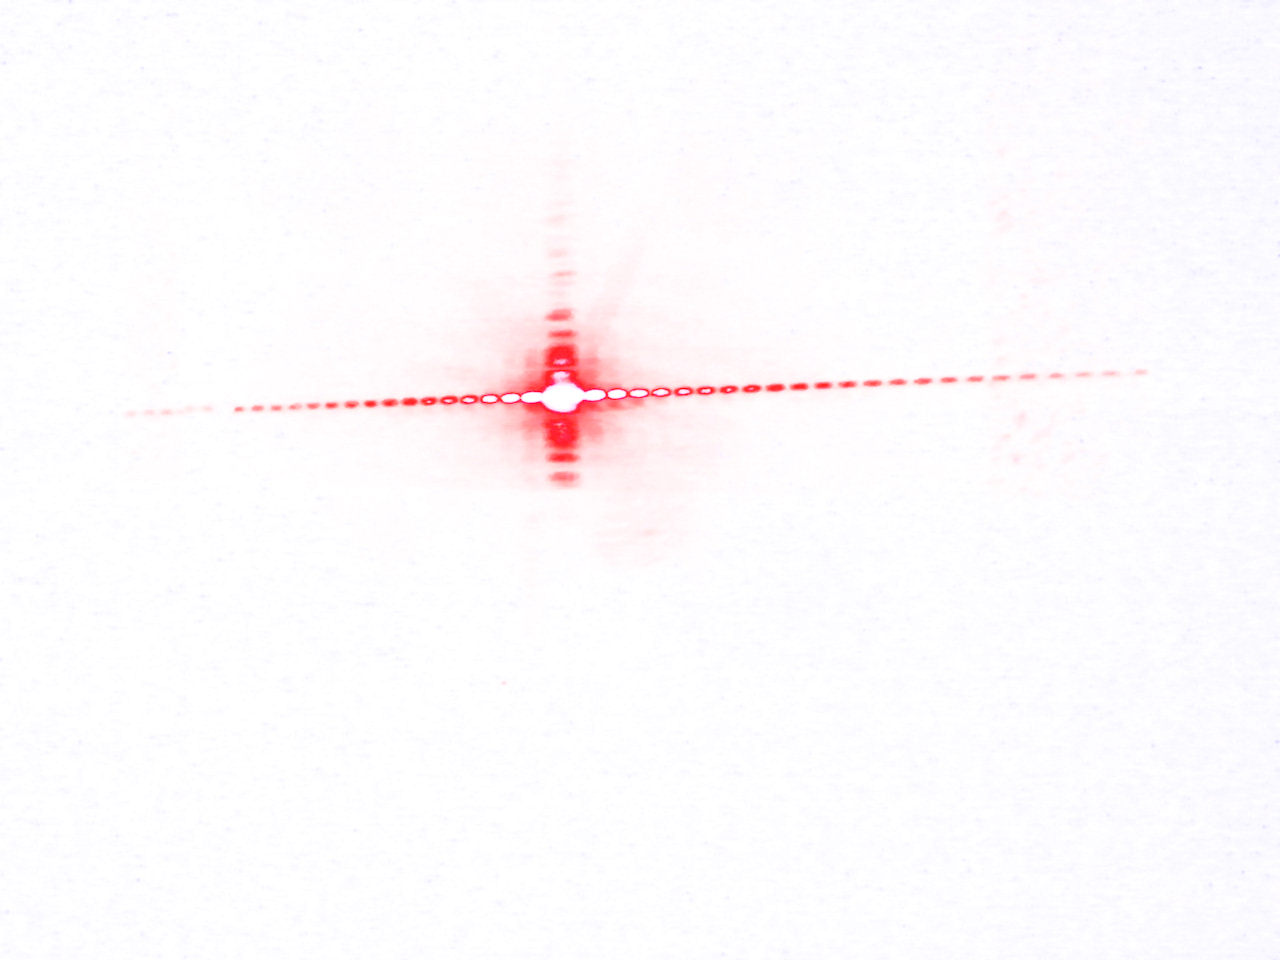
\includegraphics[scale=0.35]{./figure/beugung.png}
	\caption{Beugungsmuster Einzelspalt (echtes Foto; schwarz durch weiß ersetzt)}
	\label{fig:beugungsmuster}
\end{figure}

\begin{multicols}{2}

\section{Beugung am Spalt und Doppelspalt}
Im ersten Experiment soll ein Einzelspalt und ein Doppelspalt über die Beugung von monochromatischem Licht untersucht werden. Unsere Lichtquelle für monochromatisches Licht stellt ein Laser mit Wellenlänge $\lambda = 632.8nm$ dar. Dadurch ergibt sich ein rotes Beugungsmuster auf dem Schirm (Abb. \ref{fig:beugungsmuster}). 
\\
Durch die Vermessung des Abstandes vom Einzelspalt zum Schirm (Abb. \ref{fig:messwerte_einzelspalt}) und dem Abstand zwischen den Minima kann direkt die Spaltbreite ermittelt werden [1](Glg. 13):
$$a = \frac{n*\lambda}{sin(\alpha_{min,n})} $$
$$\alpha = arctan(\frac{b}{R})$$
b...Abstand zwischen zwei Minima\\
R...Abstand vom Spalt zum Schirm\\
\\
Beim Doppelspalt ergibt sich ein ähnliches Beugungsmuster nur das der Zentrale helle Punkt mehrere Minima und Maxima enthält. Durch eine Herleitung über die Beziehung zwischen Spaltbreite und Spaltabstand kann der Spaltabstand ermittelt werden:


%%%%%%%%%%%%%%%
$$ some formula TODO $$


%%%%%%%%%%%%%

Wesentlich in beiden Fällen ist das wir eine Fernfeldbeugung beobachten. Konkret muss der Abstand zum Beobachtungsschirm R folgender Gleichung genügen:
$$R \textgreater \frac{a^2}{\lambda}$$
wobei\\
a...Weite des Spaltes\\
$\lambda$...Wellenlänge des verwendeten Lichtes\\
\\


\subsection{Messwerte und Ergebnisse}


\end{multicols}
\begin{figure}[H]
	\centering
	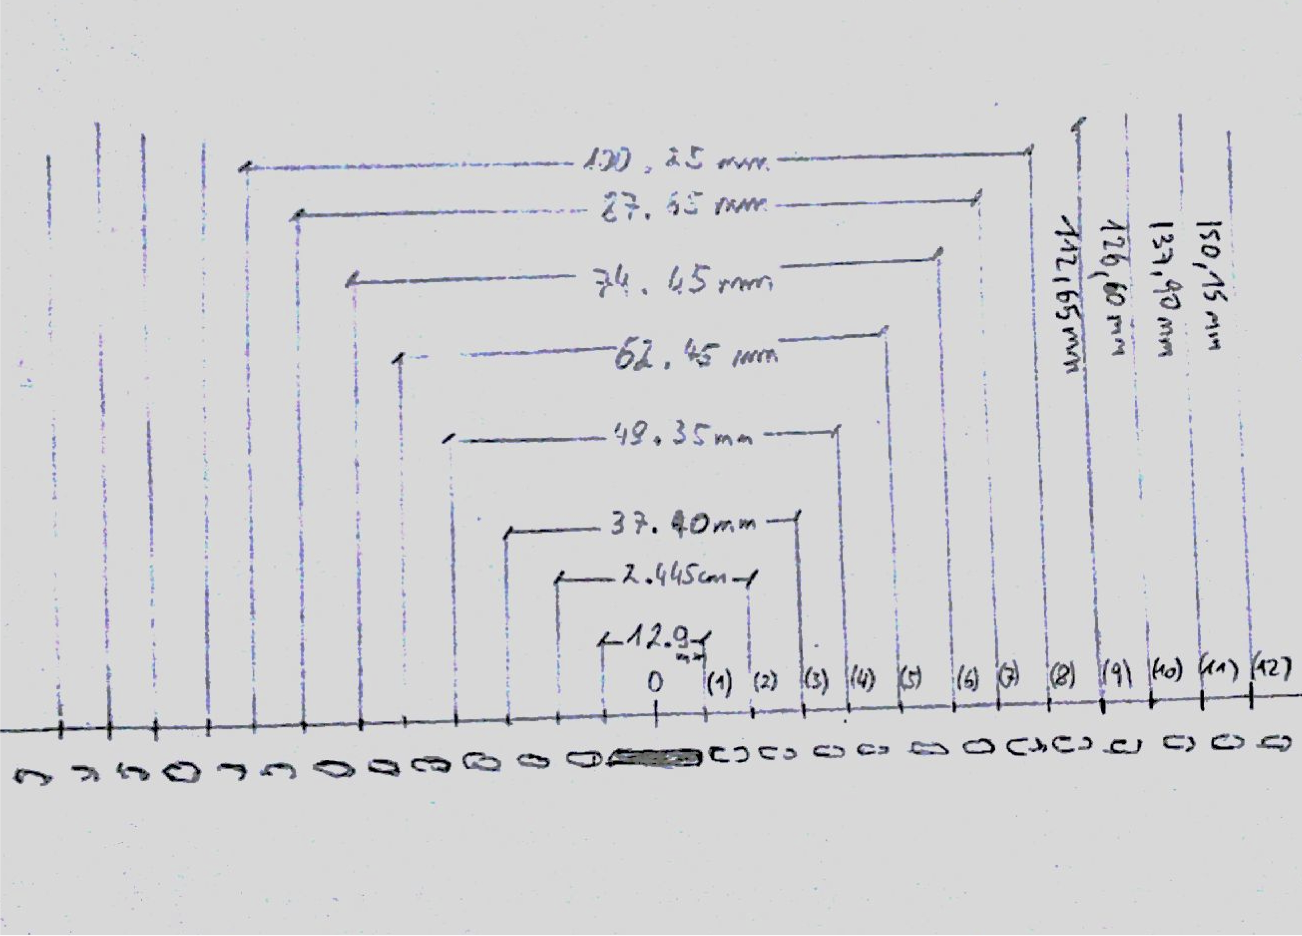
\includegraphics[scale=0.9]{./figure/einzelspalt_beugung.png}
	\caption{Beugungsmuster Einzelspalt mit Werten}
	\label{fig:messwerte_einzelspalt}
\end{figure}
\begin{figure}[H]
	\centering
	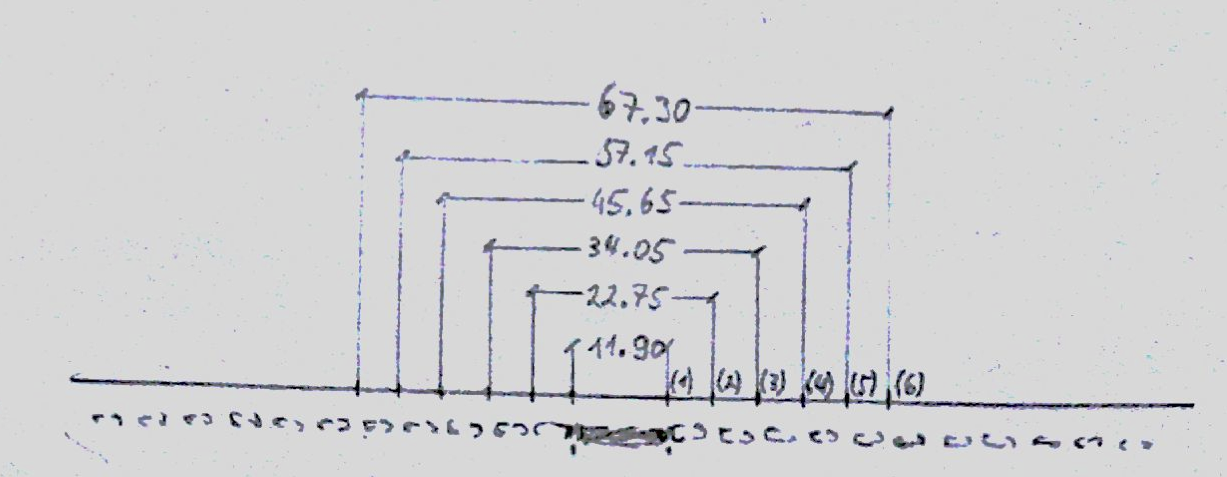
\includegraphics[scale=0.9]{./figure/doppelspalt_beugung.png}
	\caption{Beugungsmuster Doppelspalt mit Werten; ohne Minima und Maxima in der 0ten Ordnung}
	\label{fig:messwerte_doppelspalt}
\end{figure}

\begin{multicols}{2}

Tabelle, Grafik Regression, Fehlerrechnung

\subsection{Diskussion}

Wackelgeschichte, Scharfstellen, Doppelspalt-Maxima/Minima 9 statt 11

%%%%%%%%%%%%%%%%%%%%%%%%%%%%%%%%%%%%%%%%%%%%%%%%
\section{Wellenlängenmessung am Gitter}

Nachdem im 1. Versuch also die Beugungserscheinungen von Licht am Einzel- und am Doppelspalt
untersucht wurden, geht es in diesem Teil von PW8 um die Beugung am Gitter.\\
Jeder einzelne Spalt des Gitters erzeugt seine Einzelspaltbeugung, wobei Inteferenzen durch die Wellen aus all den anderen Spalten entstehen, ähnlich wie beim Doppelspalt. Im Unterschied zu diesem inteferieren nach dem Gitter jedoch Wellen aus einer sehr großen Zahl von Einzelspalten.
Daraus resultiert ein Beugungsbild von sehr schmalen, stark ausgeprägten Maxima mit sehr kleinen, praktisch dunklen, Gebieten dazwischen.\\
Durch die Beugung von Lichtstrahlen an einem Gitter soll das Spektrum einer Lampe bestimmt werden:\\
Die untersuchte Lampe strahlt nur einige bestimmte Wellenlängen ab. Da die Beugung von der Wellenlänge abhängt, werden die verschiedenen Farben unterschiedlich stark gebeugt. Durch die engen und deutlichen Beugungsmaxima, die vom Gitter verursacht werden, lassen sich die Beugungswinkel der einzelnen Farben bestimmen und ihre Wellenlänge berechnen:
$$\lambda = \sin{\alpha_{max,n}}\cdot \frac{b}{n}$$
wobei $b$ (beim Doppelspalt der Abstand zwischen beiden Spalten) hier der Gitterkonstante $g=10 \mu m$ entspricht.\\
Zur Messung der jeweiligen Winkel wird mit einem Kollimatorrohr ein Parallelstrahlenbündel durch das Gitter geschickt und die verschiedenen Beugungsmaxima mit einem Fernrohr auf einem Goniometer anvisiert.\\
%reference auf die zeichnung%
Zuerst wird die Nulllage des Systems durch Zielen auf das zentrale Maximum ermittelt. In diesem sind alle Farben der Lampe vereint, daher ist es (annähernd) weiß.\\
Es werden 3 Beugungen, jeweils links und rechts des zentralen Maximums, von insgesamt 3 Spektralfarben auf diese Art vermessen. Die Bildung des Mittelwertes ergibt schließlich die Wellenlänge der jeweiligen Farbe und, im Vergleich mit den Literaturwerten verschiedener Lampen, kann ermittelt werden, um welche Spektrallampe es sich handelt.

\subsection{Messwerte und Ergebnisse}

\begin{figure}[H]
	\centering
	\pgfplotstabletypeset[
			columns={ordnung, gruen, gelb, blau},
			col sep=&,
			columns/ordnung/.style={string type, column name=\makecell{$Ordnung$\\Maximum} }, 
			columns/gruen/.style={string type, column name=\makecell{$gruen$\\$[Grad]$\\$\pm 2'$} }, 
			columns/gelb/.style={string type, column name=\makecell{$gelb$\\$[Grad]$\\$\pm 2'$}, precision=0},
			columns/blau/.style={string type, column name=\makecell{$blau$\\$[Grad]$\\$\pm 2'$}, precision=0},
			every head row/.style={before row=\hline,after row=\hline\hline},
			every last row/.style={after row=\hline},
			every first column/.style={column type/.add={|}{} },
			every last column/.style={column type/.add={}{|} }
			]{
			ordnung & gruen & gelb & blau
			links 1: & 3$^\circ$ 8' & 3$^\circ$ 19' & 2$^\circ$ 27'
			rechts 1: & 3$^\circ$ 9' & 3$^\circ$ 21' & 2$^\circ$ 32'
			links 2: & 6$^\circ$ 17' & 6$^\circ$ 38' & 4$^\circ$ 57'
			rechts 2: & 6$^\circ$ 18' & 6$^\circ$ 39' & 5$^\circ$ 7'
			links 3: & 9$^\circ$ 26' &  &
			rechts 3: & 9$^\circ$ 27' &  &
			links 4: & & 13$^\circ$ 26' & 10$^\circ$ 0'
			rechts 4: & & 13$^\circ$ 24' & 10$^\circ$ 7'
			
			
			
						
			}
	\caption{Beugungswinkel 3er Spektralfarben, je 6 Messungen}
	\label{fig:beugungeswinkel_quecksilberspektrum}
\end{figure}


Gitterkonstante $g= 10 \mu m$

$$gruen: \lambda_{gruen}=(547.60 \pm 0.76)nm$$
$$gelb: \lambda_{gelb}=(579.9 \pm 1.5)nm$$
$$blau: \lambda_{blau}=(436.7 \pm 4.3)nm$$


\noindent Es handelt sich um eine Quecksilberdampflampe.\\
Wellenlängen (Literaturwert [2]):\\
$gruen: \lambda_{gruen}=546.07nm$\\
$gelb: \lambda_{gelb}=579.07nm$\\
$blau: \lambda_{blau}=435.83nm$\\

\subsection{Diskussion}


%%%%%%%%%%%%%%%%%%%%%%%%%%%%%%%%%%%%%%%%%%%%%%%%
\section{Newtonsche Ringe}


\subsection{Messwerte und Ergebnisse}



\subsection{Diskussion}

\section{Quellen}
$[1]$ Leitfaden, \url{http://www.univie.ac.at/anfpra/neu1/pw/pw8/PW8.pdf}\\
%$[2]$

\end{multicols}
\end{document}